\documentclass[conference,compsoc]{IEEEtran}
\bibliographystyle{IEEEtran} % We choose the "plain" reference style
\usepackage{algorithm}
\usepackage{algorithmic}
\usepackage{multirow}
\usepackage{stmaryrd}
\usepackage{amsmath}
\usepackage{amssymb}
\usepackage{enumitem}
\usepackage{subfig}
\usepackage{gensymb}
\usepackage{cite}
\usepackage{graphicx}
\usepackage{subcaption}
\usepackage{xcolor}
\usepackage{bm}

\begin{document}


\newpage
\section*{APPENDIX}

\section{Related Work}
\label{Related Work}

\subsection{Traditional Registration Methods}
As classical registration method, ICP \cite{besl1992method} iteratively updates transformation estimation by minimizing ${l_2}$ distance between registered source points given current estimation and the reference points. Variants of ICP algorithm \cite{chen1992object,trucco1999robust,chetverikov2005robust,yang2015go,koide2021voxelized} have been proposed to resist effect of outliers and speed up convergence. NDT \cite{biber2003normal} utilizes Netwon's algorithm to maximize registered points' summed probability on source points' probability density. RANSAC \cite{fischler1981random} follows a "generation and verification" scheme, where candidate correspondences are sampled and after a certain iterations, an alignment is produced based on maximum number of consensus. Many of its variants \cite{2005Matching,5459241,2018Graph} accelerate the process and improve its robustness. FGR \cite{zhou2016fast} and Teaser \cite{yang2020teaser} manage to register points by solving global optimization problem using Geman-McClure algorithm and truncated least square algorithm respectively while at higher computation cost. A more detailed review on traditional optimization based methods can be found in \cite{yang2019performance}.
 
\section{Evaluation Metrics}
\label{Evaluation Metrics}

\begin{enumerate}[label=(\alph*)]
\item \textbf{Relative Rotation and Translation Error}(RRE/RTE): the deviations from the ground-truth pose as:

\begin{equation}
RRE = \arccos(\frac{trace(\hat{\textbf{R}}^{T}{\cdot}\textbf{R}) - 1}{2})
\end{equation}

\begin{equation}
RTE = {\lVert \textbf{t} - \hat{\textbf{t}} \rVert}_{2}
\end{equation}

\item \textbf{Registration Recall} (RR): we adopt registration recall defined as the fraction of the point cloud pairs whose RRE and RTE are both below certain thresholds: for 3DMatch\&3DLoMatch benchmarks ${RRE < 15^{\circ}, RTE < 30cm}$, for KITTI odometry benchmark ${RRE < 5^{\circ}, RTE < 60cm}$. 

% Equation \ref{rr_3dmatch} denotes definition of RR for 3DMatch\&3DLoMatch benchmarks. Equation \ref{rr_kitti} denotes definition of RR for KITTI odometry benchmark.

% \begin{equation}{\label{rr_3dmatch}}
%     RR_1 = \frac{1}{M}\sum_{i=1}^{M}{\llbracket} RRE_i < 15^{\circ} \wedge RTE_i < 0.3m {\rrbracket}
% \end{equation}

% \begin{equation}{\label{rr_kitti}}
%     RR_2 = \frac{1}{M}\sum_{i=1}^{M}{\llbracket} RRE_i < 5^{\circ} \wedge RTE_i < 0.6m {\rrbracket}
% \end{equation}

\item \textbf{Inlier Ratio} (IR): it is measured by the fraction of inlier pairs among point pairs. A pair of points are inliers if the distance between transformed source point under ground truth transformation and reference point is smaller than inlier threshold ${\tau_{1}}$, which is set to 0.1m for 3DMatch\&3DLoMatch benchmarks.

\begin{equation}
   IR = \frac{1}{|\mathcal{C}|}{\sum_{(p_i^{s},p_i^{r})\in\mathcal{C}}{{\llbracket} || \textbf{R} \textbf{p}_{i}^{s} + \textbf{t} - \textbf{P}_{i}^{r}||<\tau_{1} {\rrbracket}}}
\end{equation}

\item \textbf{Feature Matching Recall} (FMR): it calculates fraction of putative pairs whose IR is above a certain threshold ${\tau_2 = 0.05}$. For the second stage of point pairs, a triplet pairs are inliers only if all three point pairs satisfy inliers requirement.

\begin{equation}
   FMR = \frac{1}{M}\sum_{i=1}^{M}{{\llbracket} IR_i > \tau_2 {\rrbracket}}
\end{equation}

\end{enumerate}

\section{Implementation Details}
\label{Implementation Details}

We implement and evaluate our model with PyTorch \cite{paszke2019pytorch} on hardware: CPU Intel i7-12700 and single GPU Nvidia RTX3090. 

For 3DMatch\&3DLoMatch benchmarks, at the first stage of triplet pairs initialization module, we select 10240 number of entries (${N_c = 10240}$) as number of candidate pairs and further filter via spatial consistency to choose 512 number of pairs (${N_g = 512}$). During flood fill process, we iterate for 120 (${\lambda_f = 120}$) number of times. We choose neighborhood size to 9 and top 1 (${N_k = 1}$) corresponding pair will be added to each group of pairs. Number of iterations ${\lambda_c}$ is set to 5. Both triangle inlier threshold ${\sigma_d}$ and inlier threshold ${\tau_s}$ are set to 0.1m. NMS distance threshold is set to 5cm and length threshold ${\sigma_l}$ is set to 0.05m.

For KITTI odometry benchmarks, since number of points for each frame is much larger and each frame covers a larger area, we increase both triangle inlier threshold ${\sigma_d}$ and inlier threshold ${\tau_s}$ to 0.6m. Length threshold ${\sigma_l}$ is also set to 0.6m. NMS distance threshold is set to 1.2m. 24 nearest neighbor points are visited. The rest parameter settings are the same as settings in 3DMatch\&3DLoMatch benchmarks.

We use a KPConv-FPN backbone extracted from GeoTransformer as our backbone for feature extraction. We follow \cite{huang2021predator,qin2022geometric} to downsample the point clouds with a voxel size of 2.5 cm on 3DMatch and 30 cm on KITTI. We keep using 4 stages KPConv-FPN layers and 5 stages KPConv-FPN layers as in \cite{qin2022geometric}. Details of configuration and training parameters can be found \cite{qin2022geometric}.

\section{High Inlier Ratio on Triplet Pairs Initialization}
In order to generate more successfully registered initial poses, more triplet correspondences should be inlier triplet correspondences. A triplet correspondences are thought to be inlier triplet correspondences when all three point pairs are inlier pairs. Based on this definition, we make analysis on triplet pairs initialization module and evaluate inlier ratio of triplet pairs. 
% For evaluating quality of generated triplet pairs, we also make ablation study on our triplet pairs initialization module. We define quality of triplet pairs by triplet inlier ratio. Specifically, a triplet pairs are thought to be inlier triplet pairs when all three point pairs are inlier pairs. 
We calculate inlier ratio per scene and visualize inlier ratio distribution through all scenes. Figure \ref{fig:triplet inlier} shows that inlier ratio has significantly declined from 3DMatch datasets to 3DLoMatch datasets since it is much harder to output inlier points on 3DLoMatch scenes. More noticeable thing from both Figure \ref{fig:triplet inlier}(a) and Figure \ref{fig:triplet inlier}(b) is, inlier ratio distributions from first stage of point pairs are very similar to the second stage of triplet pairs. It means for those of inlier point pairs, they basically "seize" the chance to find another two point pairs that are also inlier pairs. Numerically, we evaluate difference of \emph{feature matching recall} between the first stage point pairs and the second stage triplet pairs. For 3DMatch benchmark, it slightly drops from 98.2\% on first stage pairs to 97.0\% on second stage pairs and for 3DLoMatch benchmark, it drops from 87.3\% to 78.2\%. This supports our proposal that  our triangle compatibility could provide good choices on two other point pairs to form inlier triplet pairs.
% generally all scenes inlier ratio  all six points that form a triplet pairs are considered to high quality. We compare our method with DHVR \cite{lee2021deep} as both methods generate triplet pairs at early phase of registration process. For fair comparison, we also utilize FCGF descriptor, keeping it the same as DHVR. Figure \ref{fig:example} shows that inlier distribution difference between corresponding pairs and their triplet pairs on challenging 3DLoMatch \cite{huang2021predator}. And our triangle compatibility design is proved to be more capable of generating higher inlier triplet pairs than other methods.
\begin{figure}%
   \centering
   \subfloat[\centering Inlier Ratio on 3DMatch]{{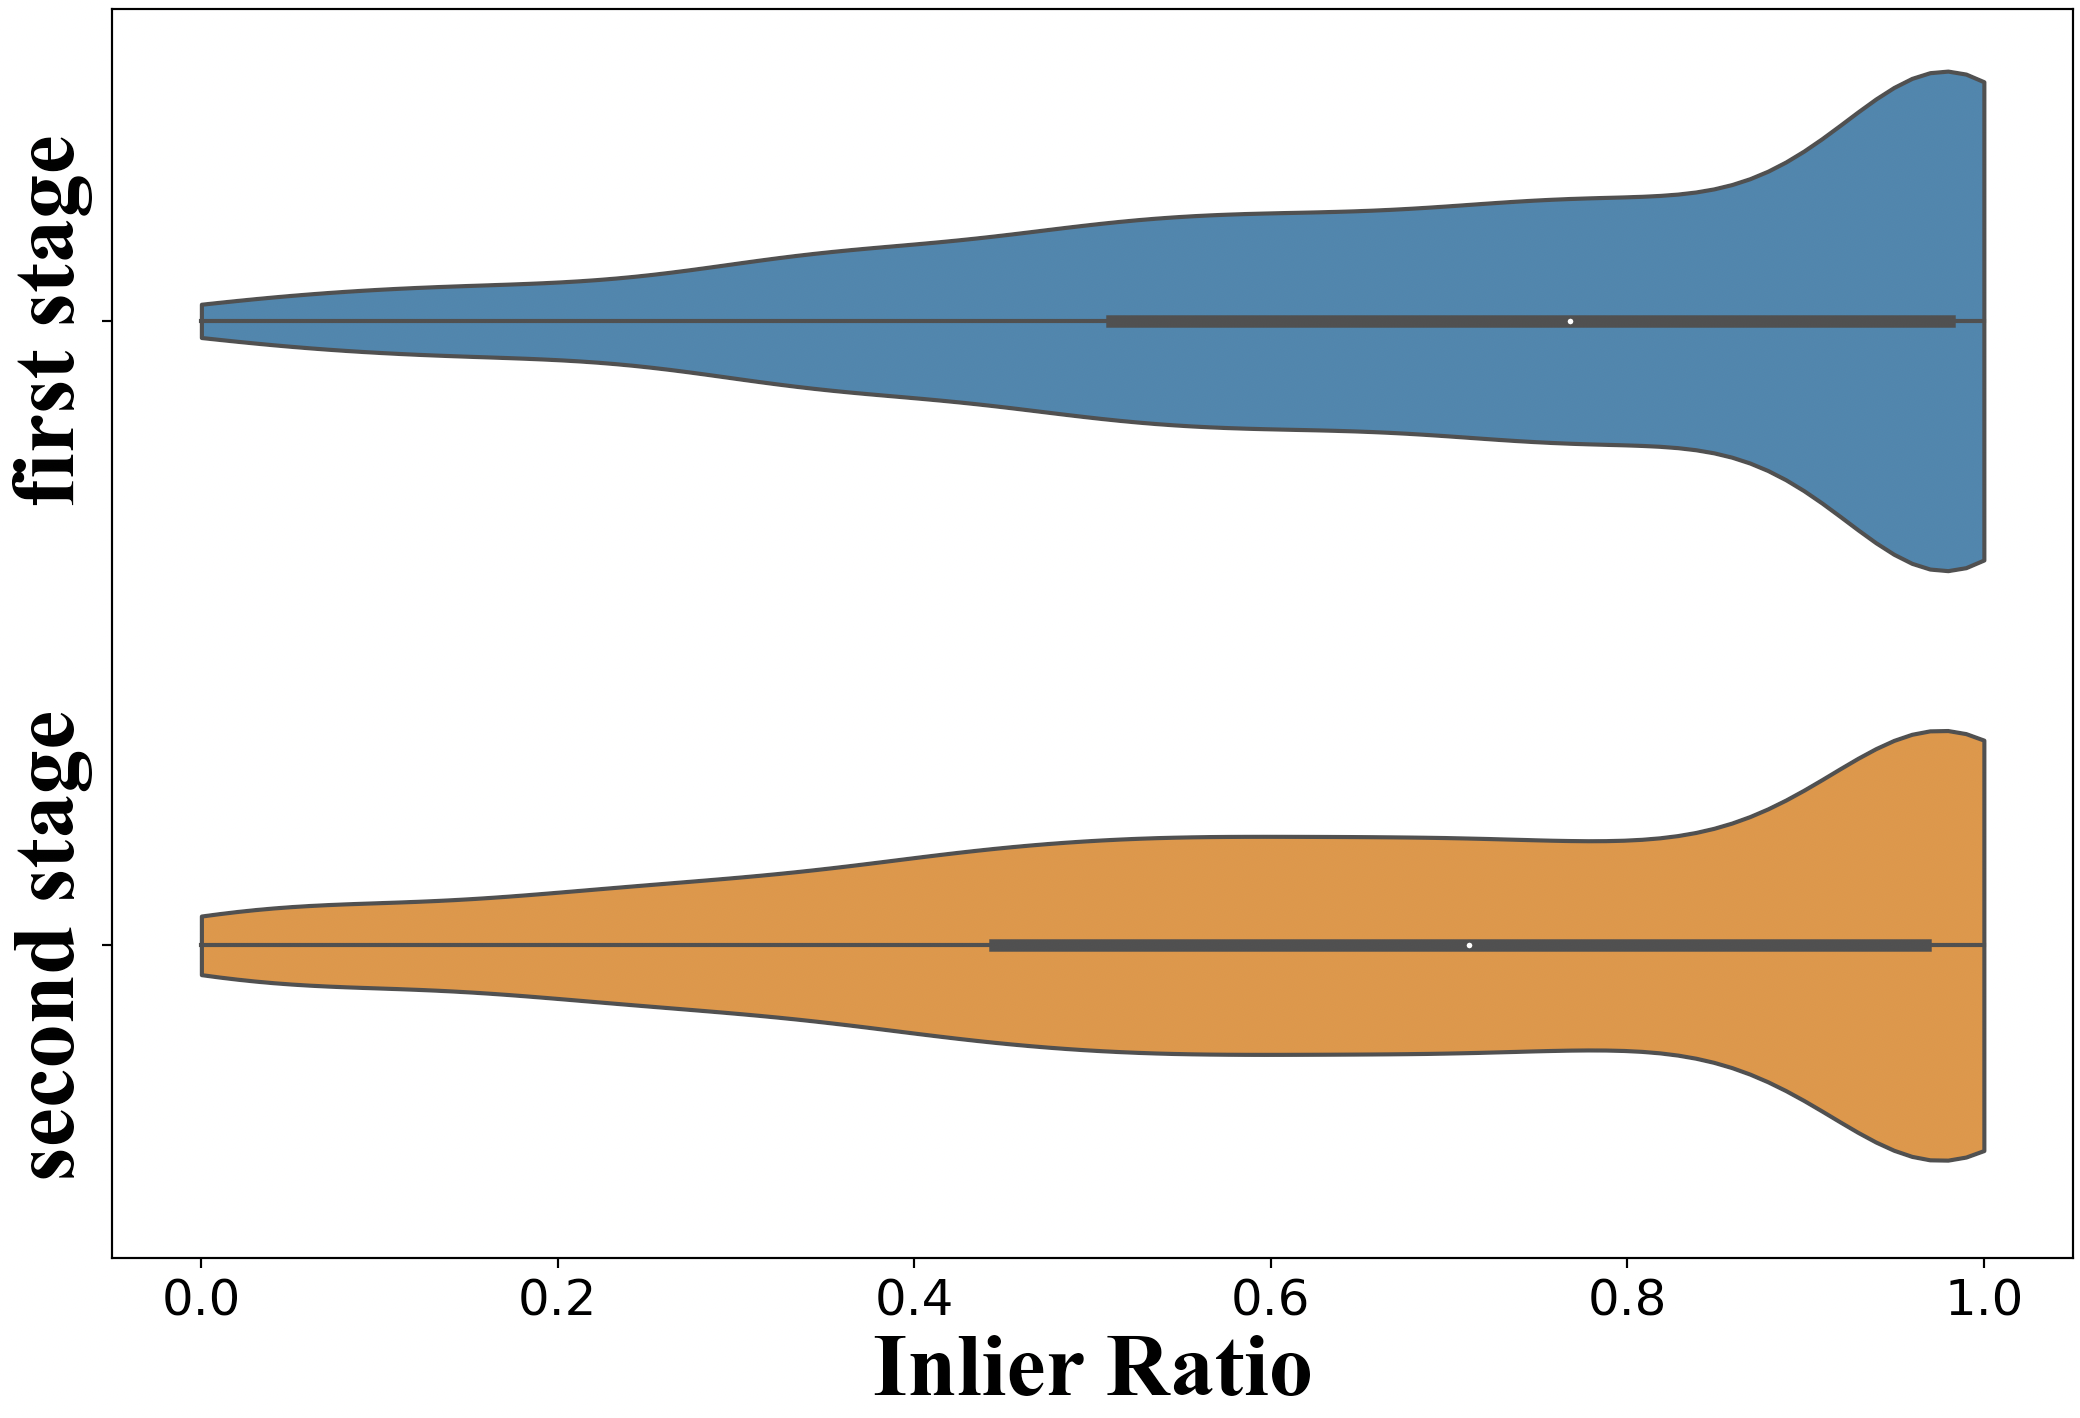
\includegraphics[width=4.0cm]{Figure/3dm_ir.png} }}%
   \hfill
   \subfloat[\centering Inlier Ratio on 3DLoMatch]{{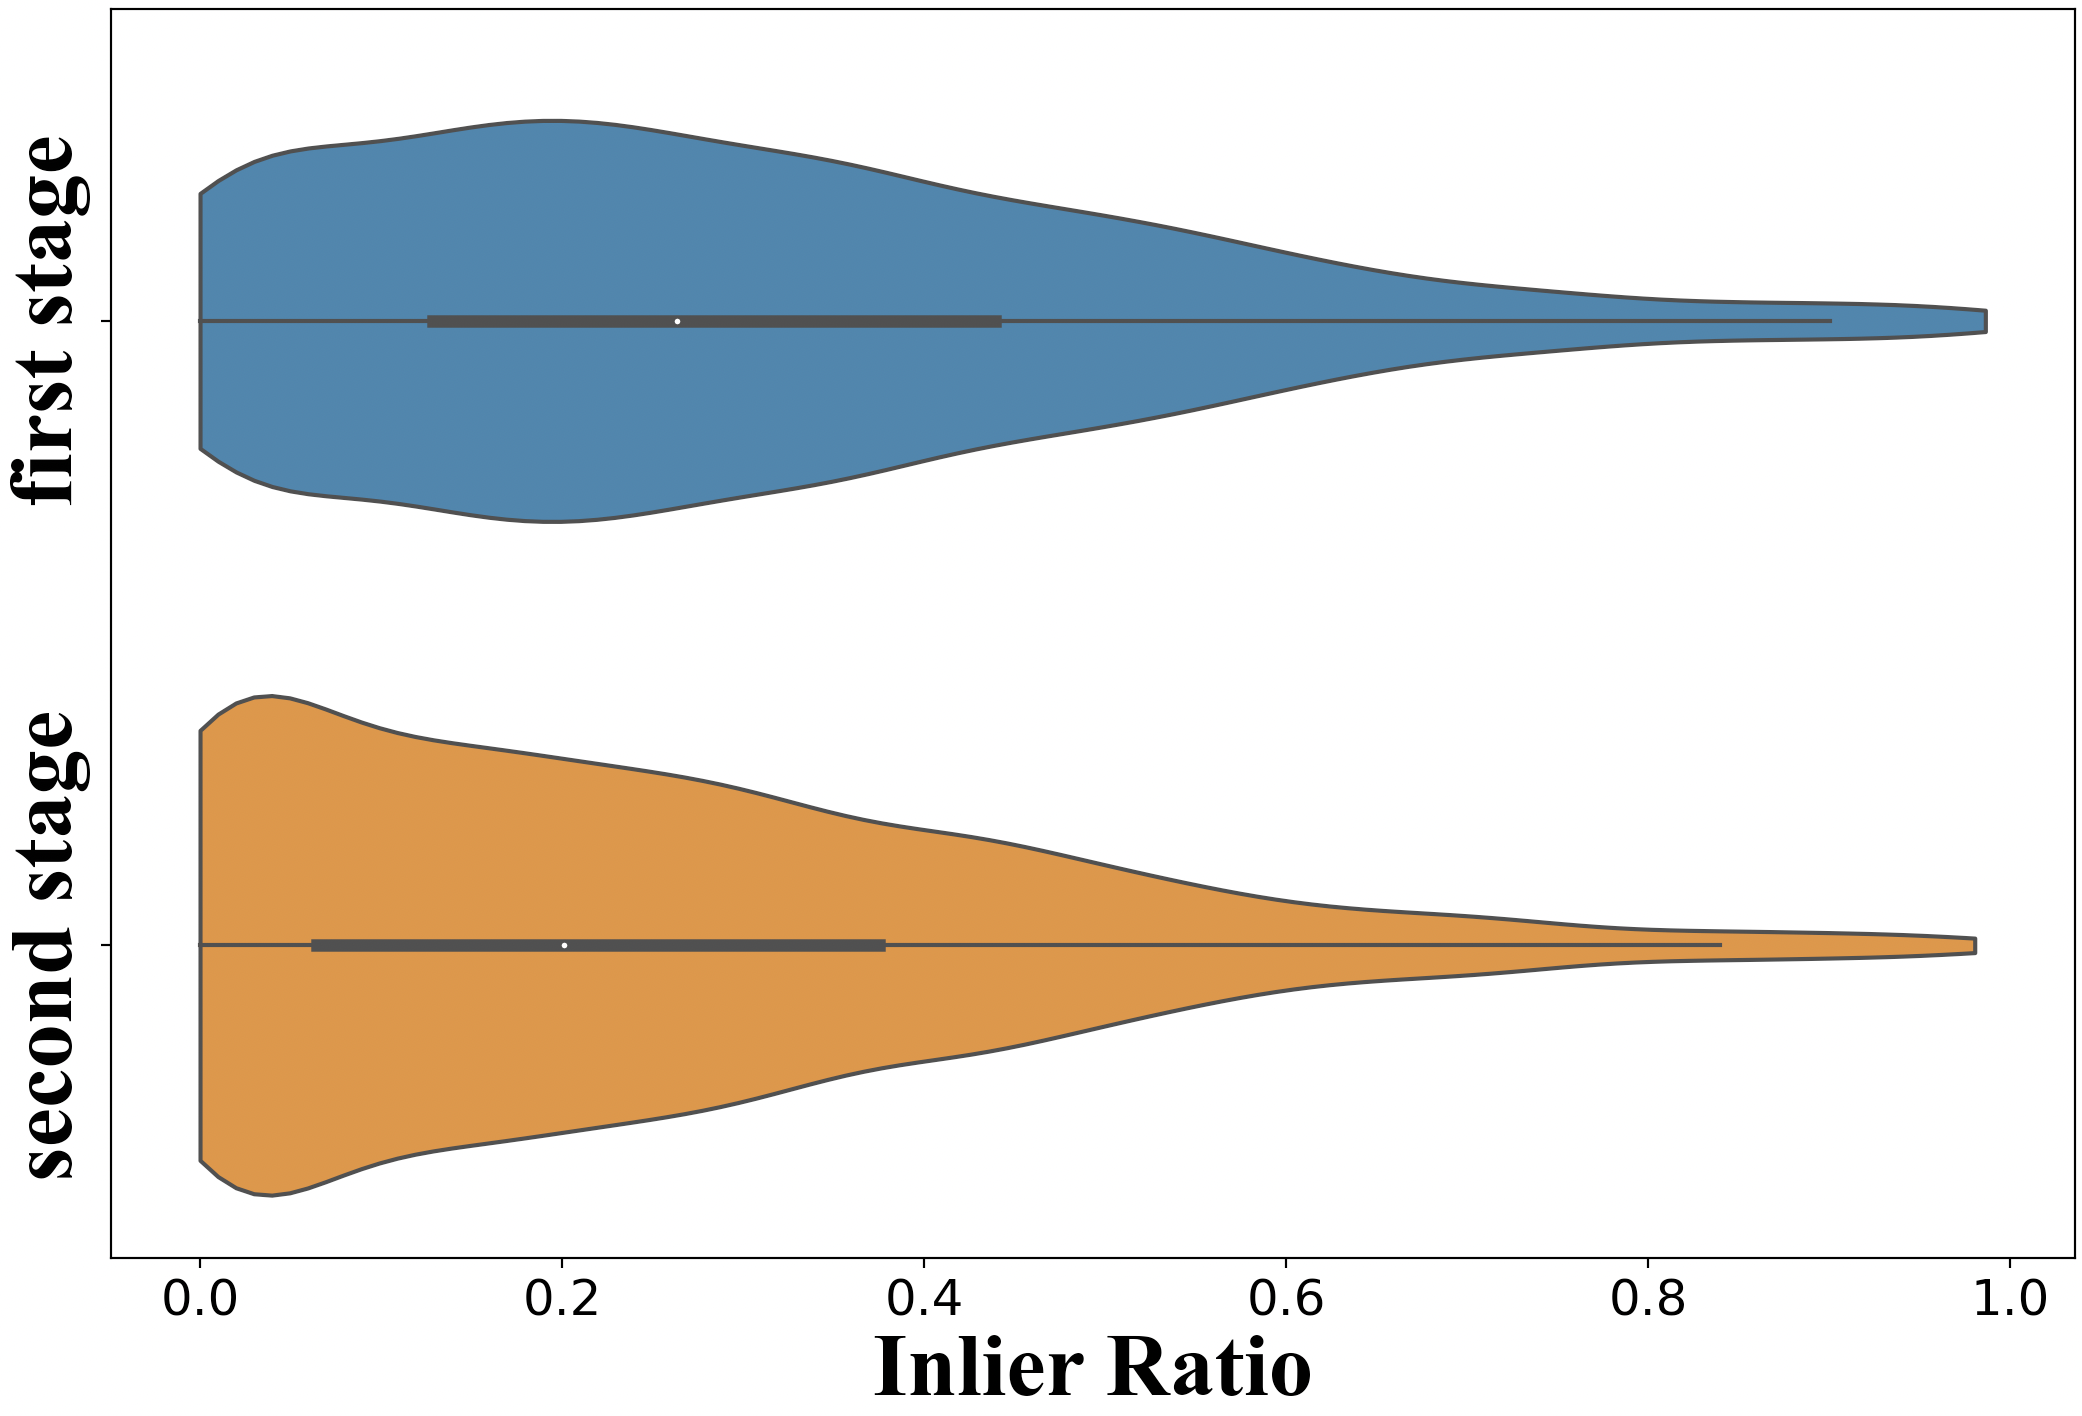
\includegraphics[width=4.0cm]{Figure/3dlm_ir.png} }}%
   \caption{Comparison between inlier ratio of first pairs and inlier ratio of triplet pairs on both 3DMatch\&3DLoMatch benchmarks. We name inlier ratio of triplet pairs as percentage of triplet pairs that all their three pairs are inlier point pairs.}%
   \label{fig:triplet inlier}%
\end{figure}

\section{Ablation Study: CRPS Module.}
\label{crps_module}
As the last step to refine correspondences and select pose, we enforce another ablation analysis on our CRPS module. We set weighted SVD \cite{umeyama1991least} as our baseline method. Weights are assigned based on Equation \ref{confidence matrix}. Then we add LGR \cite{yu2021cofinet} and RANSAC \cite{fischler1981random} as comparison. RANSAC is evaluated by point correspondences  ${\textbf{p}_f}$ obtained during first stage of triplet pairs initialization and we set iteration for sampling to be 5k. 

% We also propose a CRPS module variant: feature matching weighted CRPS, FW-CRPS in short, opts for group of pairs with largest number of consensual pairs weighted by feature scoring matching matrix ${\mathcal{C}}$ from Equation \ref{confidence matrix}.

\begin{table}[!ht]
\tiny
\begin{center}
\caption{\label{tab:ablation_estimator_exp}Evaluation Results of ablation study on Pose Estimation Strategy.}
\begin{tabular}{ p{3.0cm}|p{0.7cm}|p{0.7cm} }
\hline
\multirow{2}{*}{Estimator Module} 
& \multicolumn{2}{c}{RR(\%)} \\
& \multicolumn{1}{c}{3DMatch} & \multicolumn{1}{c}{3DLoMatch}  \\\cline{2-3}\hline\hline
Weighted-SVD \cite{umeyama1991least} & \multicolumn{1}{c}{81.45} & \multicolumn{1}{c}{32.57} \\ 
LGR \cite{yu2021cofinet} & \multicolumn{1}{c}{\underline{95.75}} & \multicolumn{1}{c}{\underline{76.98}} \\ 
RANSAC \cite{fischler1981random} & \multicolumn{1}{c}{86.69} & \multicolumn{1}{c}{40.60} \\ \hline\hline
% FW-CRPS(Ours) &  &  \\ \hline
CRPS (Ours) & \multicolumn{1}{c}{\textbf{96.12}} & \multicolumn{1}{c}{\textbf{79.06}} \\ \hline
\end{tabular}
\end{center}
% \caption{\label{tab:ablation_estimator_exp}Evaluation Results of ablation study on Pose Estimation Strategy.}
\end{table}

As shown in Table \ref{tab:ablation_estimator_exp}, our default method with CRPS module achieves highest registration result compared with other approaches. Since not all initial point pairs ${p_f}$ are inlier point pairs, non-inliers would aggregate and form group of points that are not contributing to our final pose estimation. This explains why using SVD weighted by corresponding pairs from all groups could not generate highly-successful registration. RANSAC based approach does not return accurate pose compared with LGR and our CRPS module partially due to insufficient number of corresponding pairs to sample and increasing this value should improve its performance. LGR model has been widely used by \cite{yu2021cofinet, bai2021pointdsc, qin2022geometric, chen2022sc2} and achieved competitive registration score again when added on our module. Nevertheless, our CRPS module still outperforms it.

\section{Limitations}
Despite competitive performance of our registration method, measurement of feature matching matrix from first stage of our triplet pairs initialization module might need to be adjusted according to the corresponding feature descriptor in order to maximize registration performance. Any new feature descriptor may require additional work to fine-tune the feature matching matrix to obtain higher inlier-ratio of matches with top-k (${k=N_c}$) highest scores from feature matching matrix. In the future, we will also work on designing triplet pairs initialization module that relies less on feature descriptor design.




%  \section{Second Section}

%  \section{Third Section}

%  \begin{itemize}
%     \item See Appendix \ref{FirstAppendix}
%     \item See Appendix \ref{FirstSubsectionAppendix}
%     \item See Appendix \ref{SecondAppendix}
%     \item See Appendix \ref{ThirdAppendix}
%     \item See Appendix \ref{FourthAppendix}
%   \end{itemize}

%   \begin{thebibliography}{1}
%   \bibitem{testEntry}
%       Test Ing, \emph{Testing a template}, 2017.
%   \end{thebibliography}

%   \appendices

%   \section{Related Work}
%   \label{Related Work}

%   \subsection{Traditional Registration Methods}
%   As classical registration method, ICP \cite{besl1992method} iteratively updates transformation estimation by minimizing ${l_2}$ distance between registered source points given current estimation and the reference points. Variants of ICP algorithm \cite{chen1992object,trucco1999robust,chetverikov2005robust,yang2015go,koide2021voxelized} have been proposed to resist effect of outliers and speed up convergence. NDT \cite{biber2003normal} utilizes Netwon's algorithm to maximize registered points' summed probability on source points' probability density. RANSAC \cite{fischler1981random} follows a "generation and verification" scheme, where candidate correspondences are sampled and after a certain iterations, an alignment is produced based on maximum number of consensus. Many of its variants \cite{2005Matching,5459241,2018Graph} accelerate the process and improve its robustness. FGR \cite{zhou2016fast} and Teaser \cite{yang2020teaser} manage to register points by solving global optimization problem using Geman-McClure algorithm and truncated least square algorithm respectively while at higher computation cost. A more detailed review on traditional optimization based methods can be found in \cite{yang2019performance}.
 
%   \section{Evaluation Metrics}

%   \begin{enumerate}[label=(\alph*)]
%   \item \textbf{Relative Rotation and translation Error}(RRE/RTE): the deviations from the ground-truth pose as:

%   \begin{equation}
%     RRE = \arccos(\frac{trace(\hat{\textbf{R}}^{T}{\cdot}\textbf{R}) - 1}{2})
%   \end{equation}

% \begin{equation}
%     RTE = {\lVert \textbf{t} - \hat{\textbf{t}} \rVert}_{2}
% \end{equation}

% \item \textbf{Registration Recall} (RR): we adopt registration recall defined as the fraction of the point cloud pairs whose RRE and RTE are both below certain thresholds: for 3DMatch\&3DLoMatch benchmarks ${RRE < 15^{\circ}, RTE < 30cm}$, for KITTI odometry benchmark ${RRE < 5^{\circ}, RTE < 60cm}$. Equation \ref{rr_3dmatch} denotes definition of RR for 3DMatch\&3DLoMatch benchmarks. Equation \ref{rr_kitti} denotes definition of RR for KITTI odometry benchmark.

% \begin{equation}{\label{rr_3dmatch}}
%     RR = \frac{1}{M}\sum_{i=1}^{M}{\llbracket} RRE_i < 15^{\circ} \wedge RTE_i < 0.3m {\rrbracket}
% \end{equation}

% \begin{equation}{\label{rr_kitti}}
%     RR = \frac{1}{M}\sum_{i=1}^{M}{\llbracket} RRE_i < 5^{\circ} \wedge RTE_i < 0.6m {\rrbracket}
% \end{equation}

% \item \textbf{Inlier Ratio} (IR): it is measured by the fraction of inlier pairs among point pairs. A pair of points are inliers if the distance between transformed source point under ground truth transformation and reference point is smaller than inlier threshold ${\tau_{1}}$, which is set 0.1m for 3DMatch\&3DLoMatch benchmarks.

% \begin{equation}
%     IR = \frac{1}{|\mathcal{C}|}{\sum_{(p_i^{s},p_i^{r})\in\mathcal{C}}{{\llbracket} || \textbf{R} \textbf{p}_{i}^{s} + \textbf{t} - \textbf{P}_{i}^{r}||<\tau_{1} {\rrbracket}}}
% \end{equation}

% \item \textbf{Feature Matching Recall} (FMR): it calculates fraction of putative pairs whose IR is above a certain threshold ${\tau_2 = 0.05}$. For the second stage of point pairs, a triplet pairs are inliers only if all three point pairs satisfy inliers requirement.

% \begin{equation}
%     FMR = \frac{1}{M}\sum_{i=1}^{M}{{\llbracket} IR_i > \tau_2 {\rrbracket}}
% \end{equation}

% \end{enumerate}

% \section{Implementation Details}

% We implement and evaluate our model with PyTorch \cite{paszke2019pytorch} on hardware: CPU Intel 12700 and GPU Nvidia RTX3090. For 3DMatch\&3DLoMatch benchmarks, we set 512 for number of seed triplet pairs ${N_g}$, 30 for iterations ${N_\tau}$, 12 for KNN neighbor search range, 5 for number of iterations ${N_{ts}}$ during CRPS module, 0.1m for inlier threshold ${\sigma_{d}}$, 0.1m for NMS Module distance threshold and 5cm for matching radius to evaluate inlier ratio. As number of KITTI odometry points for each frame is much larger, we increase ${L_\tau}$ to 32 and search range K to 24, we keep setting of ${N_\tau}$ the same as 512 and number of iterations ${N_{ts}}$ as 5. We assign inlier threshold for CRTS Module to 0.6m, NMS Module distance threshold to 0.6m and matching radius to evaluate inlier ratio to 60cm. We use a KPConv-FPN backbone extracted from GeoTransformer as our backbone for feature extraction. We follow \cite{huang2021predator,qin2022geometric} to downsample the point clouds with a voxel size of 2.5cm on 3DMatch and 30cm on KITTI. We keep using 4 stages KPConv-FPN layers and 5 stages KPConv-FPN layers as in \cite{huang2021predator,qin2022geometric}. Details of configuration and training parameters can be found \cite{qin2022geometric}.

%   \section{Second Appendix}
%   \label{SecondAppendix}

%   \section{Third Appendix}
%   \label{ThirdAppendix}

%   \section{Fourth Appendix}
%   \label{FourthAppendix}
 
 \bibliography{ref.bib} % Entries are in the refs.bib file

 \end{document}